\section{Background}
\label{sec:intro}
\begin{figure}[tb]
	\vspace{-10pt}
	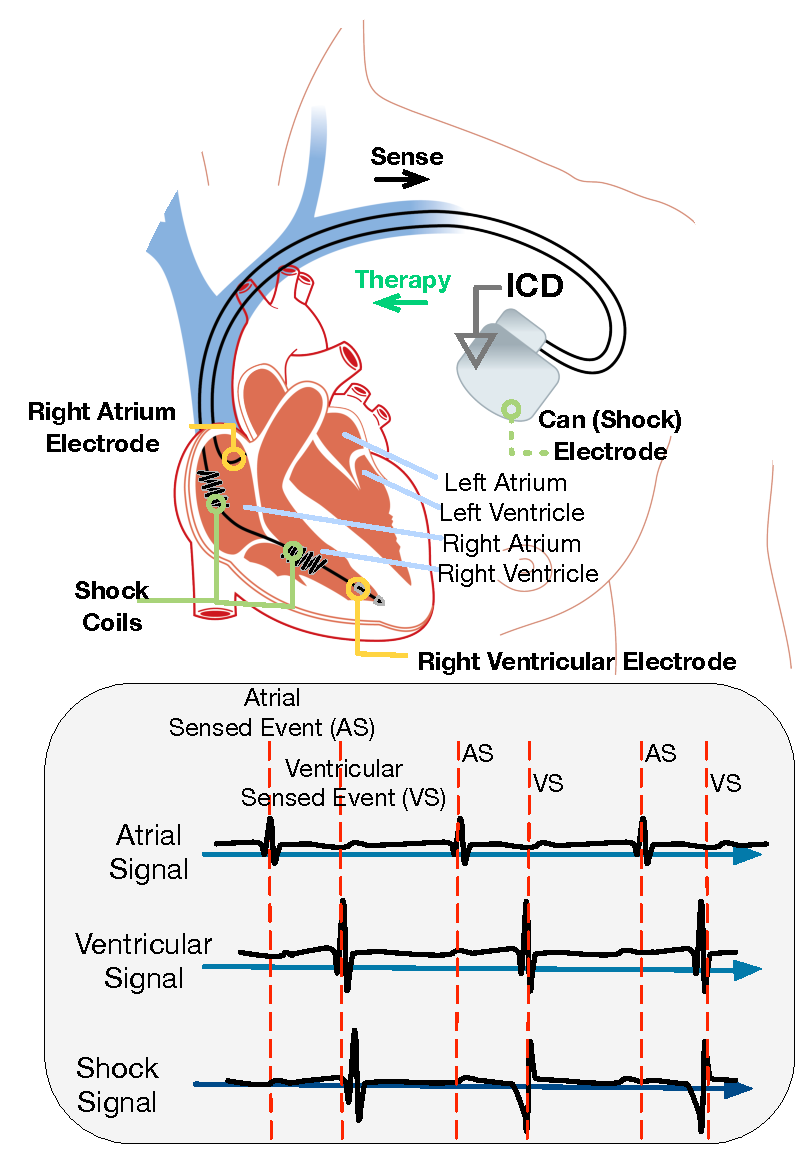
\includegraphics[scale=0.4]{figures/figICD.pdf}
	\vspace{-10pt}
	\smallcaption{ICD connected to the heart. The atrial, ventricular, and shock electrogram signals are measured by the device, which uses them to diagnose the current state of the heart and determine whether therapy is required.}
	\vspace{-10pt}
	\label{fig:icd}
\end{figure}


	\begin{figure}[t]
		\centering
		\vspace{-10pt}
		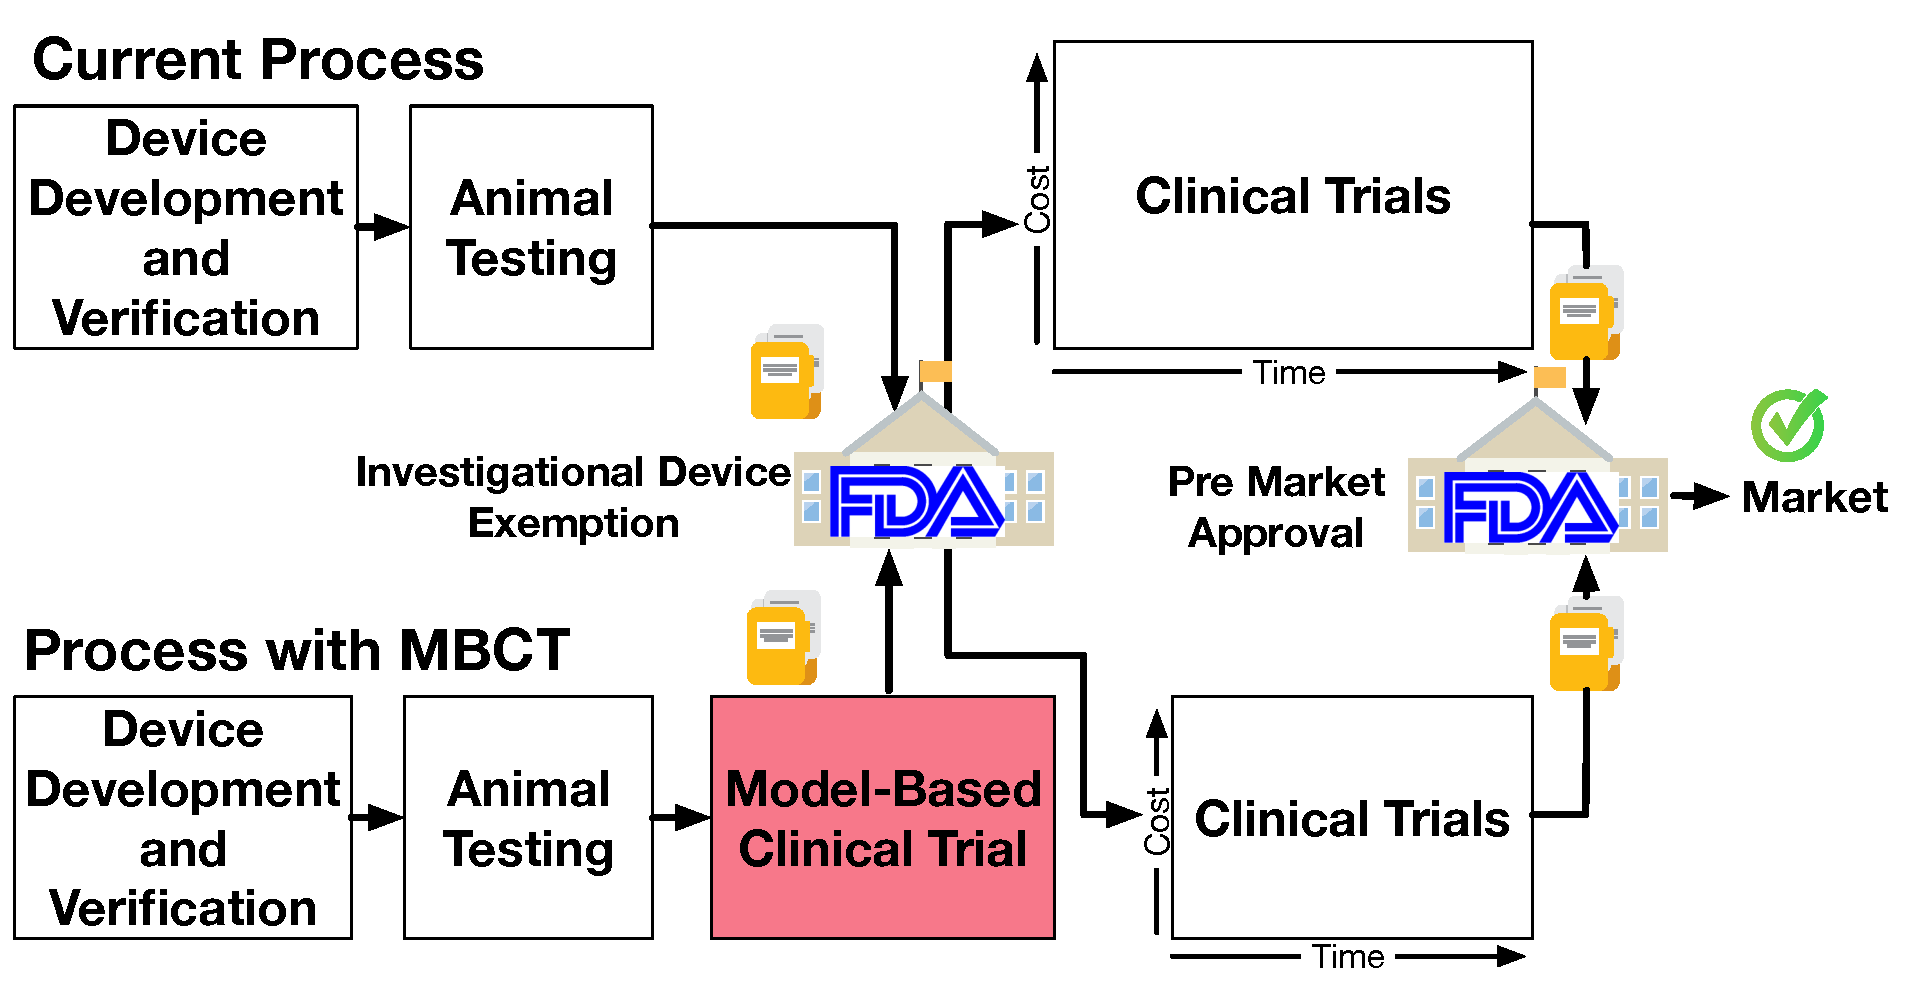
\includegraphics[scale=0.25]{figures/figTransResearchSpectrum.pdf}
		\vspace{-10pt}
		\caption{\small Bringing a device to market.			
			Model-based clinical trials will provide insight during planning and execution of clinical trials, increasing the chance of a successful trial.}
		\vspace{-10pt}
		\label{fig:spectrum}
	\end{figure}

\acp{ICD} treat the symptoms of fatal tachycardias by applying therapy to suspected episodes of sustained \ac{VT} or \ac{VF} (Fig. \ref{fig:icd}).
Therapy takes the form of a high-energy electric shock or a sequence of low-energy electric pulses.
The Rhythm ID Going Head to Head Trial (RIGHT) \cite{GoldABBTB11_RIGHTresults} sought to compare the VT/SVT discrimination abilities of two competing detection algorithms from two ICD manufacturers \cite{GoldABBTB11_RIGHTresults}: 
the detection algorithm found in Boston Scientific's Vitality II ICDs (which uses the Rhythm ID discriminators~\cite{compass}),
and the PR Logic + Wavelet detection algorithm found in a number of Medtronic's ICDs.
%The investigators chose the following primary question: is there a difference in time-to-first inappropriate therapy between the two ICDs?
\emph{Inappropriate therapy} was defined as therapy applied to an arrhythmia other than \ac{VT} or \ac{VF}.
RIGHT enrolled 1962 patients and ran for approximately five years.
It was fully sponsored by Boston Scientific. 

One of the trial's assumptions, for the purposes of sample size calculation, was that Boston Scientific's algorithm would reduce the risk of inappropriate therapy by 25\% over Medtronic's algorithm~\cite{Berger06_RIGHT}.
The outcome of the trial~\cite{GoldABBTB11_RIGHTresults}, however, was that patients implanted with Boston Scientific \acp{ICD} had a \emph{34\% risk increase} of inappropriate therapy as compared to patients implanted with Medtronic ICDs. 

Computer models of the human heart's function have been developed, with different models focusing on different aspects of the cardiac function.
In particular, electrophysiological (EP) models simulate the electrophysiological function of the heart: how depolarization is initiated in and spreads throughout the myocardium, causing contractions of the muscle.
We demonstrate how these models can assist in planning and executing clinical trials, by providing early, affordable and reproducible testing of a clinical trial's premises and assumptions (Fig. \ref{fig:spectrum}).
Model-based empirical validation of the premises reduces the risk of conducting a trial that fails to demonstrate the desired effect (typically, an improvement of new intervention over the control). 
